\begin{comment}
	\pagebreak
\end{comment}

\section{Convolutional Neural Network}
\textbf{Generalization:} trade-off specifity vs. invariance\\
\begin{comment}
	We need to trade-off specifity and invariance (created by affine transformations of an object and different lightings) to increase the generalization ability of the model.
\end{comment}

\textbf{Receptive Field:} area triggering neuron, inhibit or excit\\
\begin{comment}
	\Note{Areas can be on the Retina, Skin, Tounge, etc.}\\
	From Hubel and Wiesels experiments we learned that stimulus covering the whole cat retina, most neurons didn't fire, since the excitatory and inhibitory stimulus canceled each other out. 
	The light must fall on specific regions to excite, forming specific excitement \textit{patterns}.\\
	\textbf{Direction and alignment} of the light affected the firing, and was used to figure out the alignment of the receptive field.\\
\end{comment}

\textbf{Hierarchy:} \textbf{S}imple cells, specific stimuly, \textbf{C}omplex cells, complex stimuly\\
\begin{comment}
	\Note{Size of receptive fields tends to get larger, the more complex the cell becomes.}\\
	Sensory receptors connected to cell in the brain form the receptive field of that cell. This receptive field can be very noisy in simple cells.\\
	The connection of such simple cells to complex cells can form complex triggering patterns, f.e. a line in a certain direction.\\
	This hierarchy can be extended to hypercomplex shapes.\\
	
	\begin{Figure}
 		\centering
 		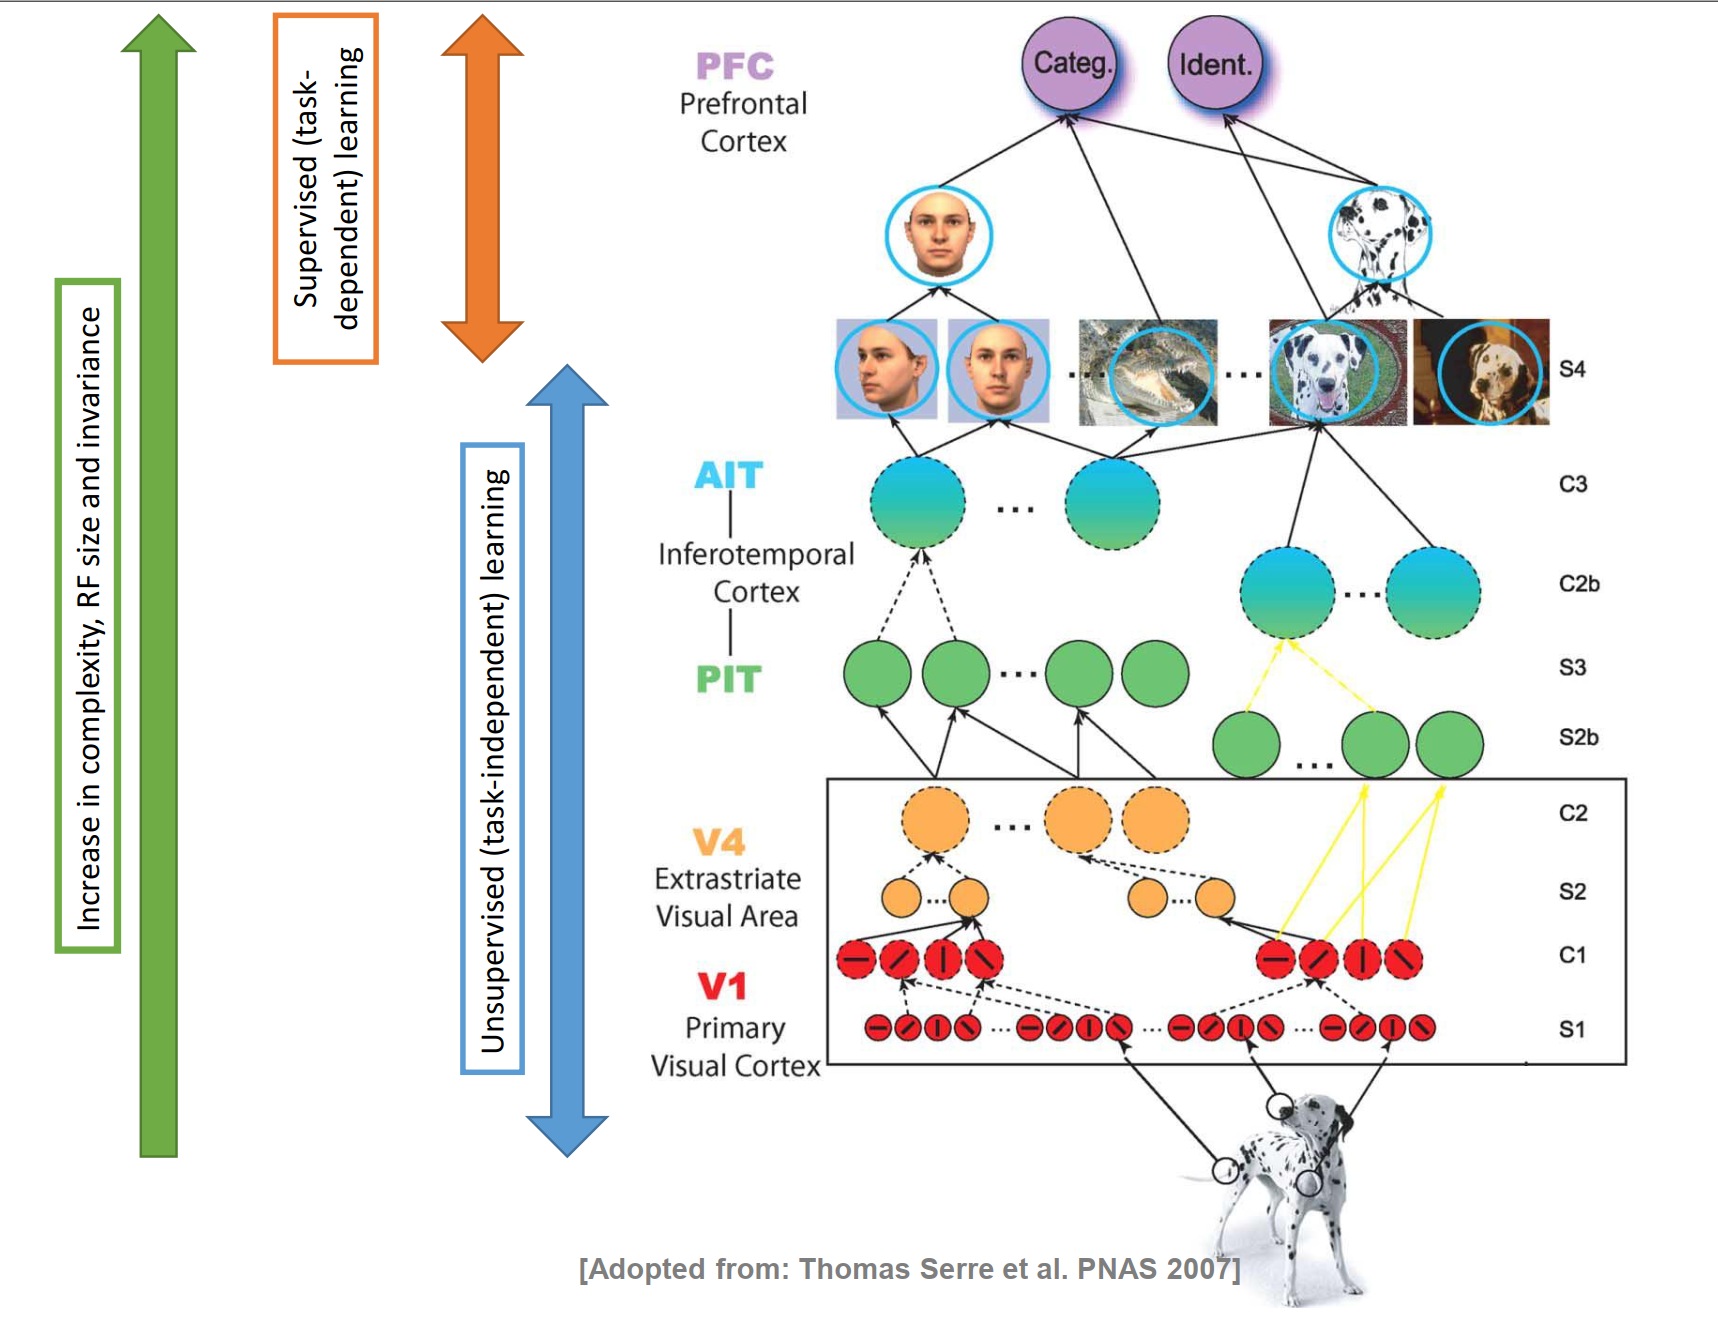
\includegraphics[width=\linewidth]{graphic/cnn-receptive-field-complexity}
 		\captionof{figure}{Complexity, unsupervised and supervised learning hierarchy}
	\end{Figure}
\end{comment}

\textbf{HMAX:} S: $y = \exp(- \frac{1}{2\sigma^2} \sum^{n_{S_k}} (w_j - x_j)^2)$, C: $y = \max_{n_{C_k}} y_j$\\
\begin{comment}
	The HMAX model is used to describe how our visual system works, it uses a hierarchical structure.
	x is the input to the cell, w is the weight of the cell, sigma is the size of the receptive field of a cell.\\
\end{comment}

\begin{comment}
	\Note{Any linear, shift-equivariant transform can be written as convolution.}\\
\end{comment}
\textbf{Linear:} $T(\alpha u + \beta v) = \alpha T(u) + \beta T(v)$\\
\textbf{Invariant:} $T(f(u)) = T(u)$\\
\begin{comment}
	\Note{We want this in classification, b.c. a cat in the middle of the picture should still be classified as cat if it is shifted or roted}\\
\end{comment}
\textbf{Equivariant:} $T(f(u)) = f(T(u))$\\
\begin{comment}
	\Note{In Edge detection very important, if we shift the edge in the image, we also want the response to shift the same way}\\
\end{comment}

\textbf{Correlation:} $I'(i,j) = \sum_{m = -k}^k \sum_{n	 = -k}^k K(m,n) I(i+m, j+n)$\\
\begin{comment}
	\Note{I is the image, K is the Kernel, N(i,j) is the neighbourhood of a pixel.}\\
	\textbf{Shift-invariance:} The Kernel is usually parameterized as K(i,j,m,n), e.g. the weights of the Kernel depend on the location in the image. Removing i,j-dependence makes the kernel shift invariant.\\
	
	\begin{Figure}
 		\centering
 		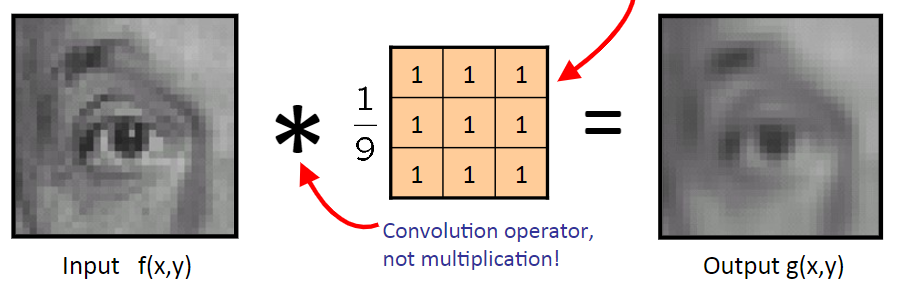
\includegraphics[width=\linewidth]{graphic/cnn-linear-filtering}
 		\captionof{figure}{Linear filtering is applied with the convolution operator to compute a new image from the neigbourhood of each pixel of the old image}
	\end{Figure}
\end{comment}

\textbf{Conv:} $I'(i,j) = \sum_{m = -k}^k \sum_{n= -k}^k K(m,n) I(i-m, j-n)$\\
\begin{comment}
	Alternative representation would be \\
	$I'(i,j) = \sum_{m = -k}^k \sum_{n = -k}^k K(-m,-n) I(i+m, j+n)$\\
	Convolution acts as a point-spread function, what we want to learn are the weights of the kernel.
	It can be done via matrix multiplication.\\
	\textbf{Correlation = Convolution:} iff $K(i,j) = K(-i, -j)$\\
\end{comment}

\textit{Ex:} rotate K by 180 to Y, $\frac{\partial E}{\partial X} = \frac{\partial E}{\partial Y} \star K$, $\frac{\partial E}{\partial K} = rot(\frac{\partial E}{\partial Y} \star X)$ \\

\textbf{Matrix $I * K$:} band matrix $K \in \R^{n+m-1 \times n}$, $k_i$ on diagonal\\
\begin{comment}
		\begin{Figure}
 		\centering
 		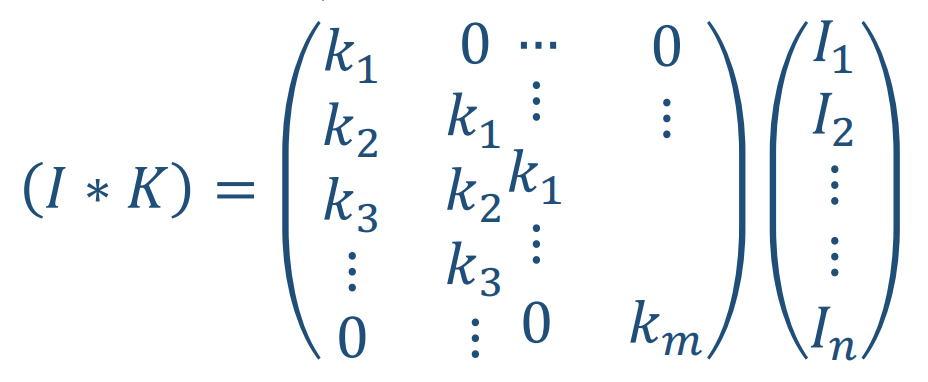
\includegraphics[width=\linewidth]{graphic/cnn-conv-matrix}
 		\captionof{figure}{CNN Convolution as matrix}
	\end{Figure}
\end{comment}

\textbf{Diff.:} Conv. with kernel [-1, 1], $\frac{\delta f}{\delta x} \approx \frac{f(x_{n+1}, y) - f(x_n, y)}{\Delta x}$\\


\textbf{Dimension:} $\frac{I_{height} + 2 \cdot \text{padding} - \text{dilation} \cdot (K_{height} - 1) - 1}{\text{stride}} + 1$\\

\begin{comment}
	\Note{If we have 6 filters, the produced "new image" would be of size 28x28x6}\\
	
	\begin{Figure}
 		\centering
 		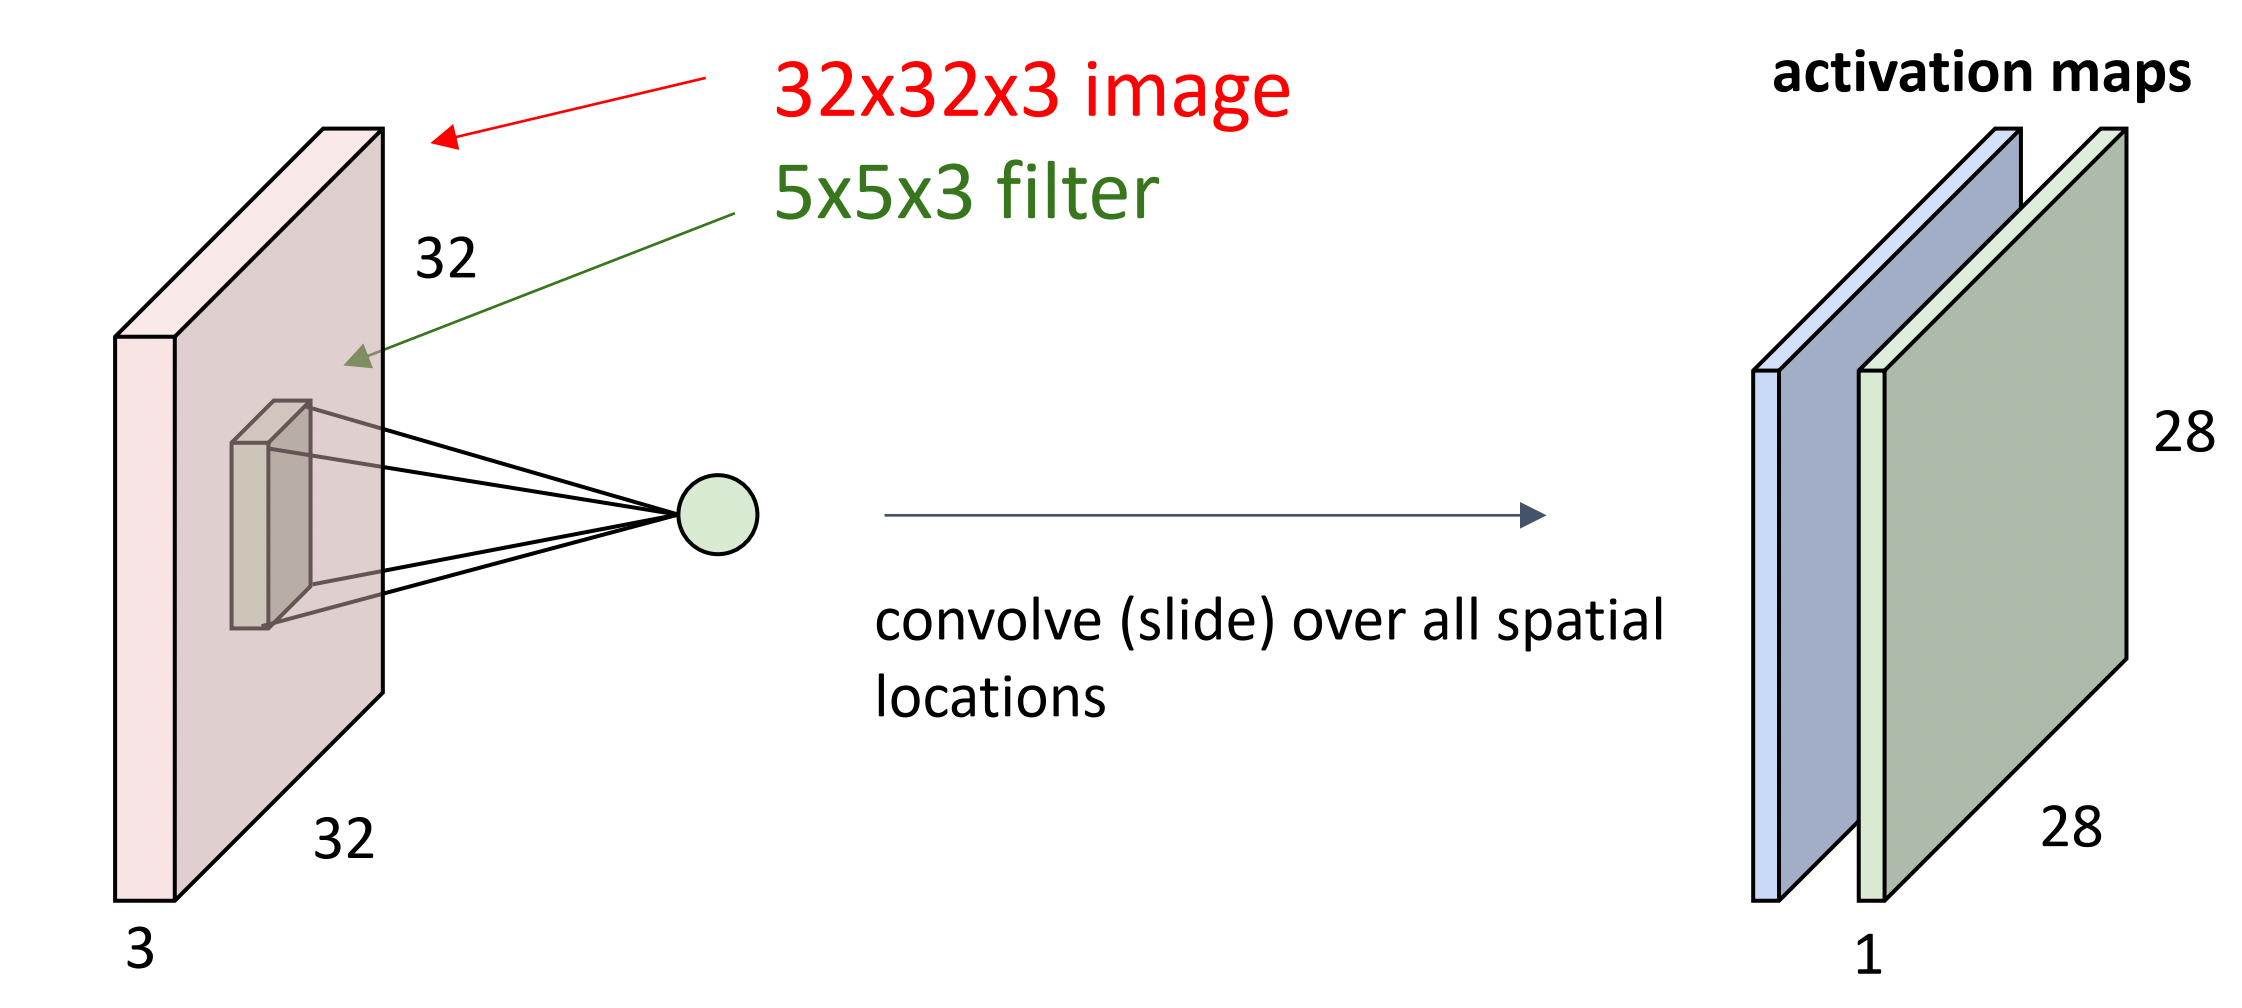
\includegraphics[width=\linewidth]{graphic/cnn-conv-layer}
 		\captionof{figure}{Visualisation applying filters to an image}
	\end{Figure}
\end{comment}

\textbf{Weight sharing:} Same K for whole I, local not global\\
\begin{comment}
	\Note{This makes the feature detector robust agains affine transformations, as it detects the feature in the whole image once trained}\\
\end{comment}

\textbf{Stride:} used to reduce size, replaces pooling layers\\
\textbf{Dillation:} fast increase of rec. field, get global context\\

\textbf{CNN-fwd:} $z_{i,j}^{(l)} = w^{(l)} * z^{(l-1)} + b = (\sum_{m,n} w_{m,n}^{(l)} z_{i-m, j-n}^{(l-1)}) + b$
\begin{comment}
	\begin{Figure}
 		\centering
 		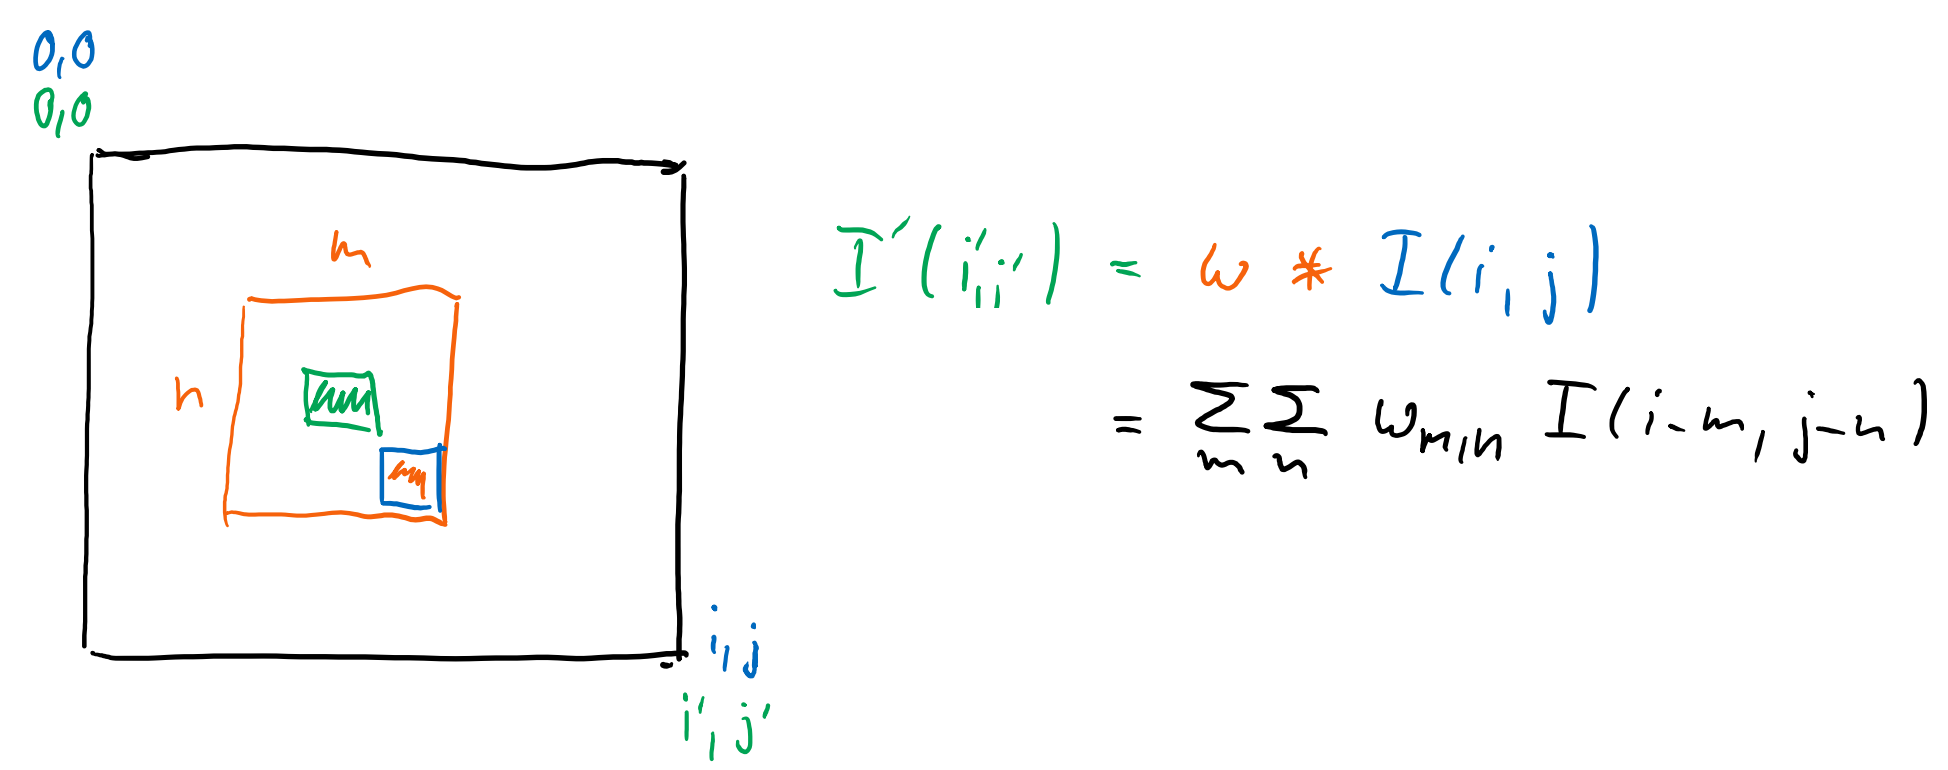
\includegraphics[width=\linewidth]{graphic/cnn-forward-pass}
 		\captionof{figure}{Visualisation forward pass}
	\end{Figure}
\end{comment}

\textbf{CNN-bwd (z):} $\delta_{i,j}^{(l-1)} 
= \frac{\delta C}{\delta z_{i,j}^{(l-1)}} 
= \sum_{i', j'} \frac{\delta C}{\delta z_{i',j'}^{(l)}} \frac{\delta z_{i',j'}^{(l)}}{\delta z_{i,j}^{(l-1)}} \\
= \sum_{i', j'} \delta_{i',j'}^{(l)} w_{i'-i,j'-j}^{(l)}
= \delta_z^{l} * ROT_{180}(w^{(l)})$\\
\begin{comment}
	If we take the derivative of $\delta z_{i',j'}^{(l)}$, only certain weight terms stick, the rest is going to be zero.\\
	\Note{Backward path is just a convolution with the flipped kernel}\\
	\begin{Figure}
 		\centering
 		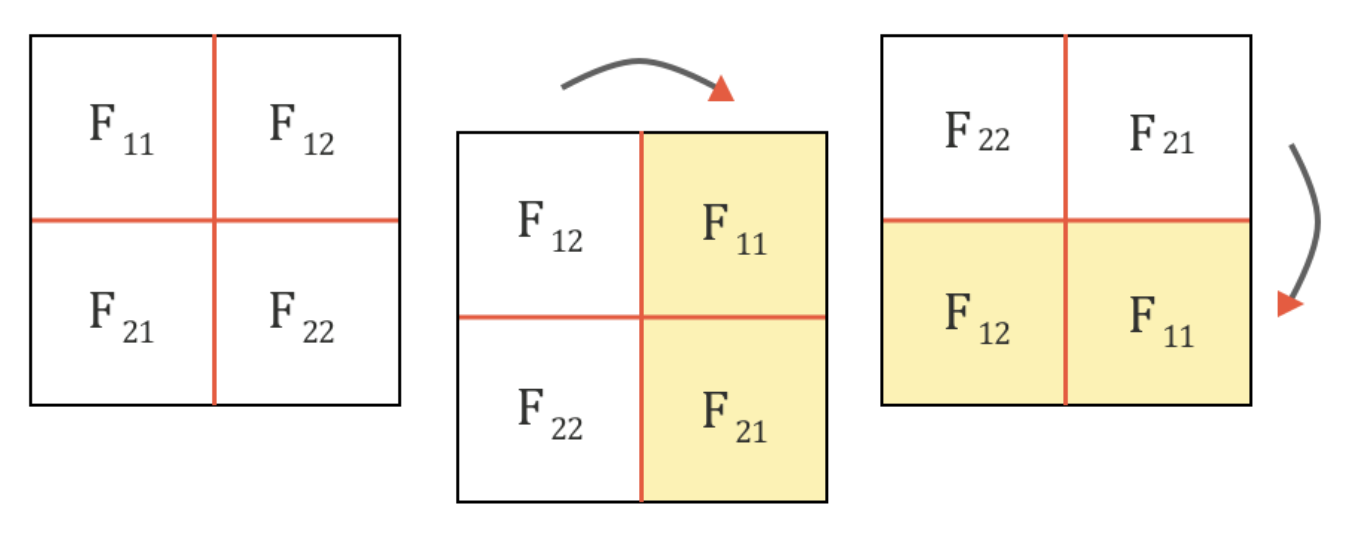
\includegraphics[width=\linewidth]{graphic/cnn-flipped-conv}
 		\captionof{figure}{Flipped convolution operator}
	\end{Figure}
\end{comment}

\begin{comment}
	\Note{Each layer holds more complex "patterns", this resembles the neuron complexity hierarchy we have seen in nature.}\\
	\begin{Figure}
 		\centering
 		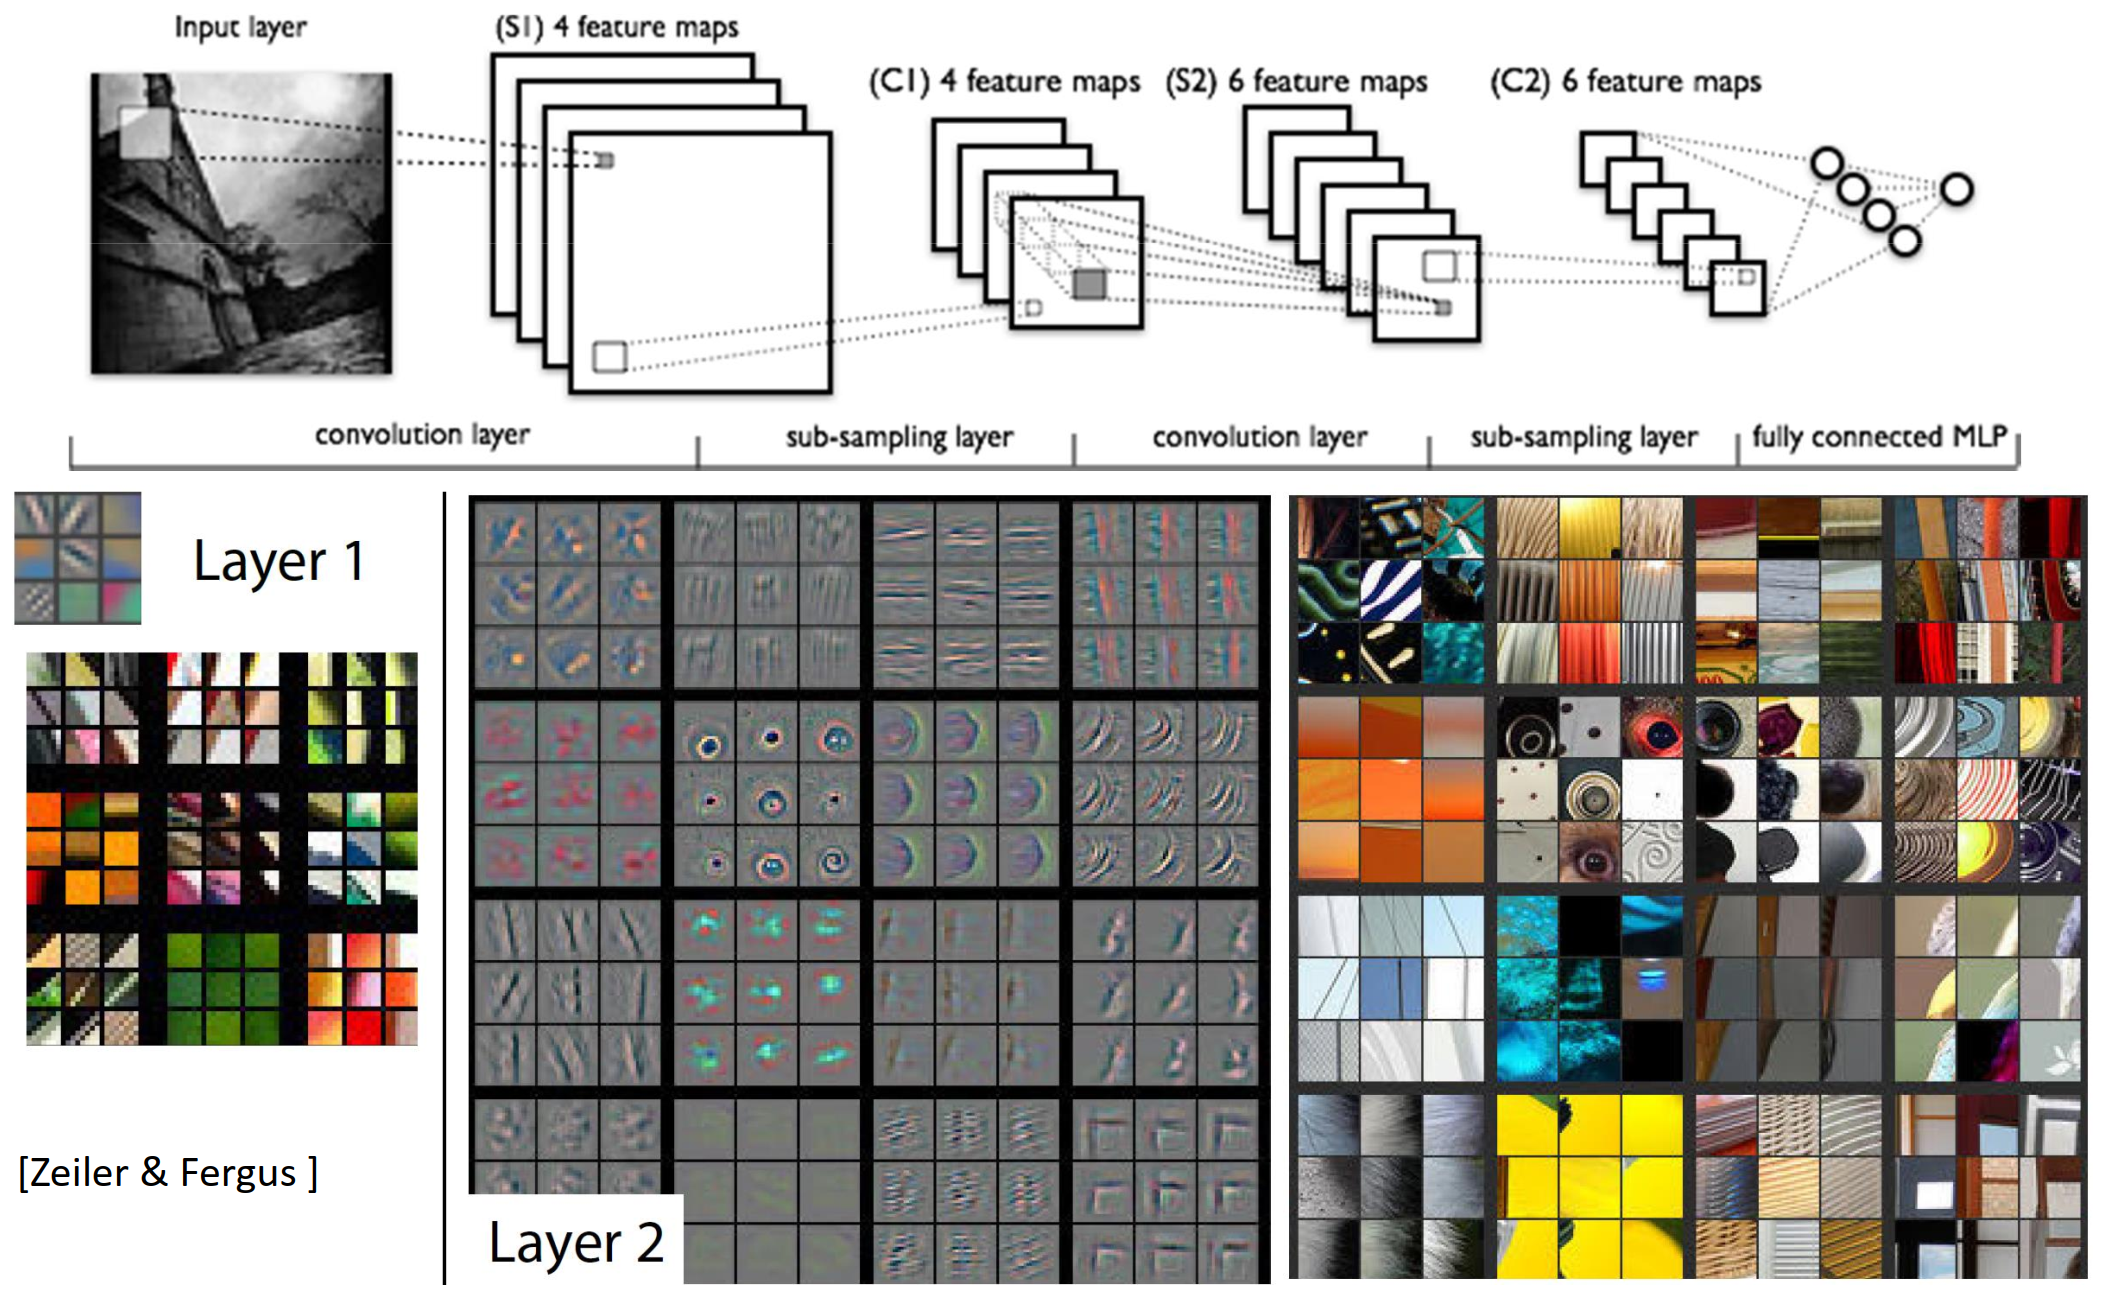
\includegraphics[width=\linewidth]{graphic/cnn-visualization}
 		\captionof{figure}{Visualisation of output of cnn layers}
	\end{Figure}
\end{comment}

\textbf{Pooling:} $z^{l} = \max\{ z_i^{l-1}\}$, $\frac{\partial z^{l}}{\partial z_i^{l-1}} = 1$ if was max else $0$\\
\begin{comment}
	Reduces size of each activation layer, downsampling. This helps in extending the activation region of downstream pixels, as we are putting more info in a smaller region. It also helps in reducing the noise in pictures.\\
	There are other pooling strategies that can be applied, but with the MAX-pooling, we gain robustness to local changes. For example, if a digit rotates a bit, the region probably still has the same max pixel and thus is robust against rotations.\\
	
	\begin{Figure}
 		\centering
 		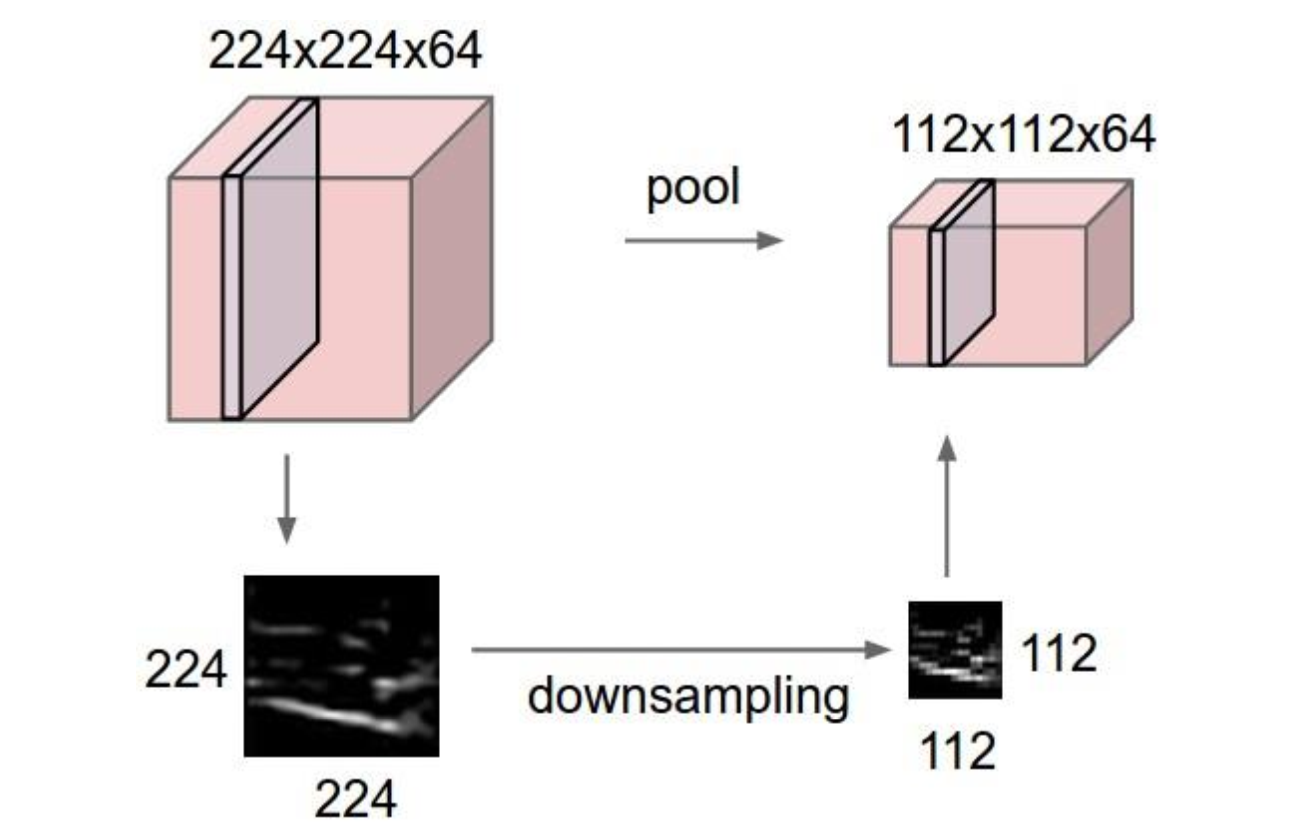
\includegraphics[width=\linewidth]{graphic/cnn-pooling-layer}
 		\captionof{figure}{Visualisation of pooling layer}
	\end{Figure}
	\begin{Figure}
 		\centering
 		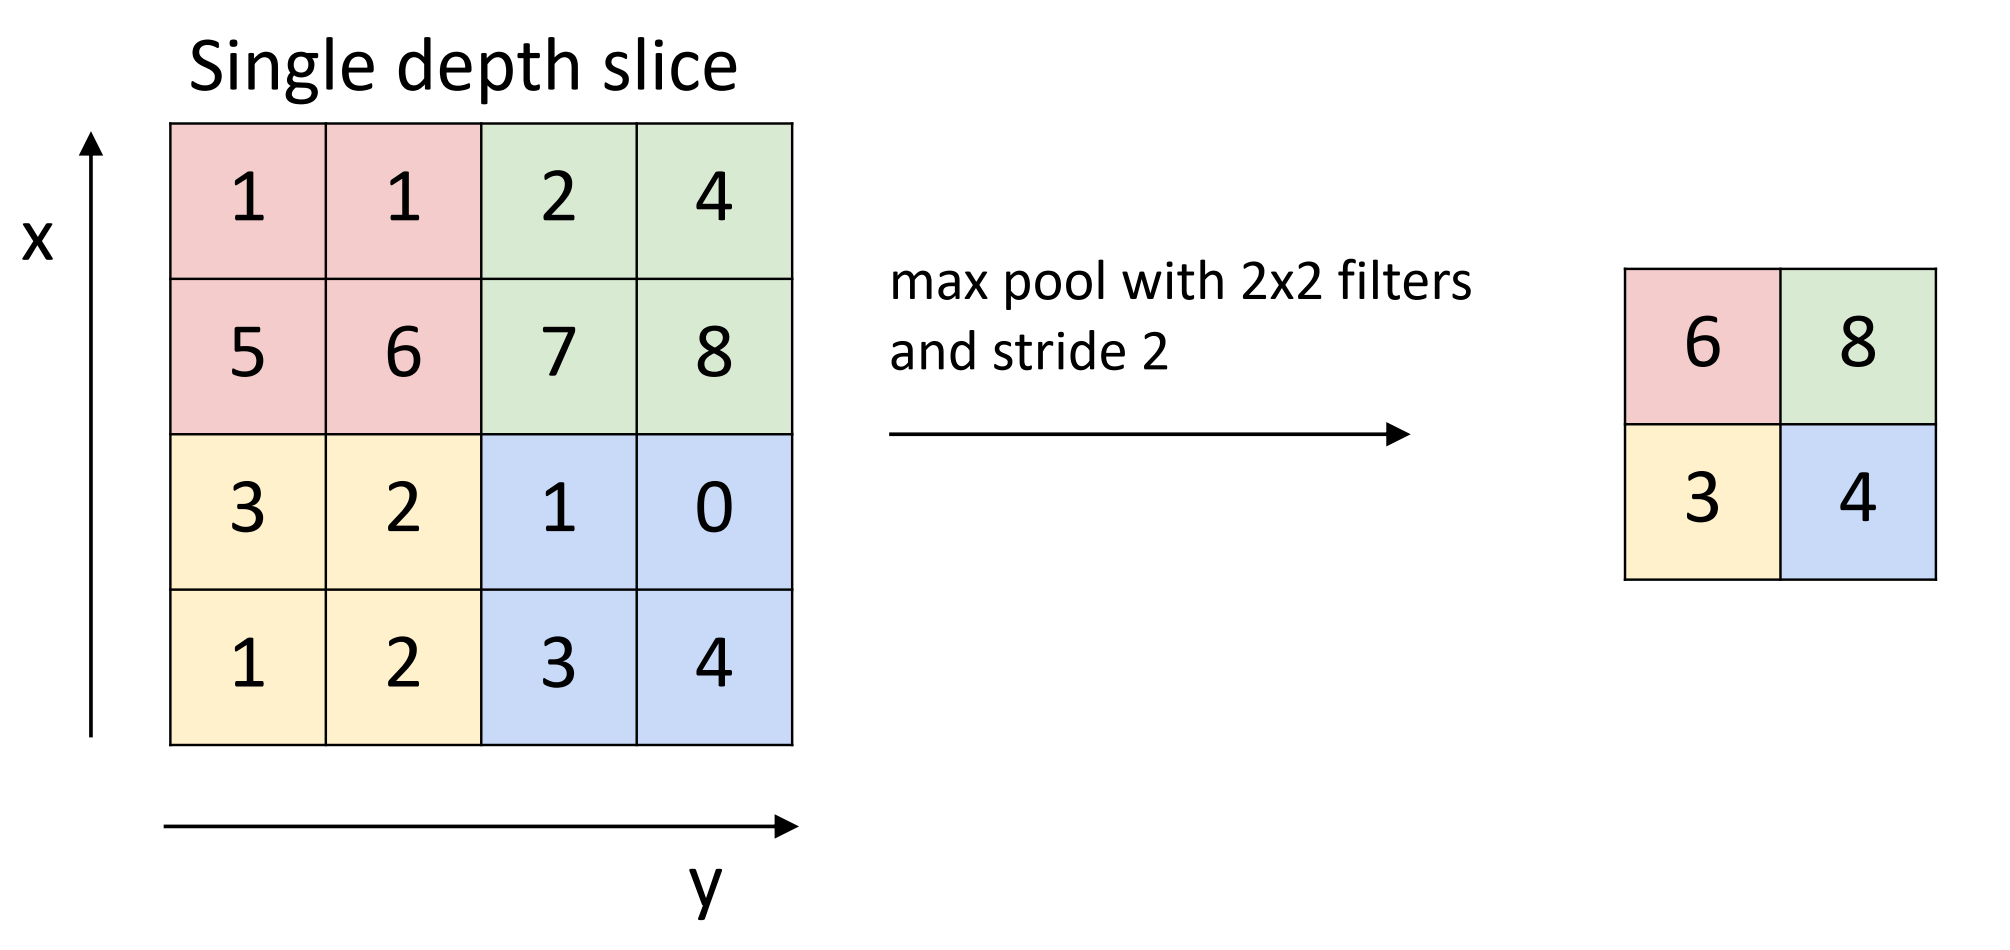
\includegraphics[width=\linewidth]{graphic/cnn-max-pooling}
 		\captionof{figure}{Visualisation of max pooling layer}
	\end{Figure}
\end{comment}

\subsection{Evolution of architectures}
\begin{comment}
	\begin{Figure}
 		\centering
 		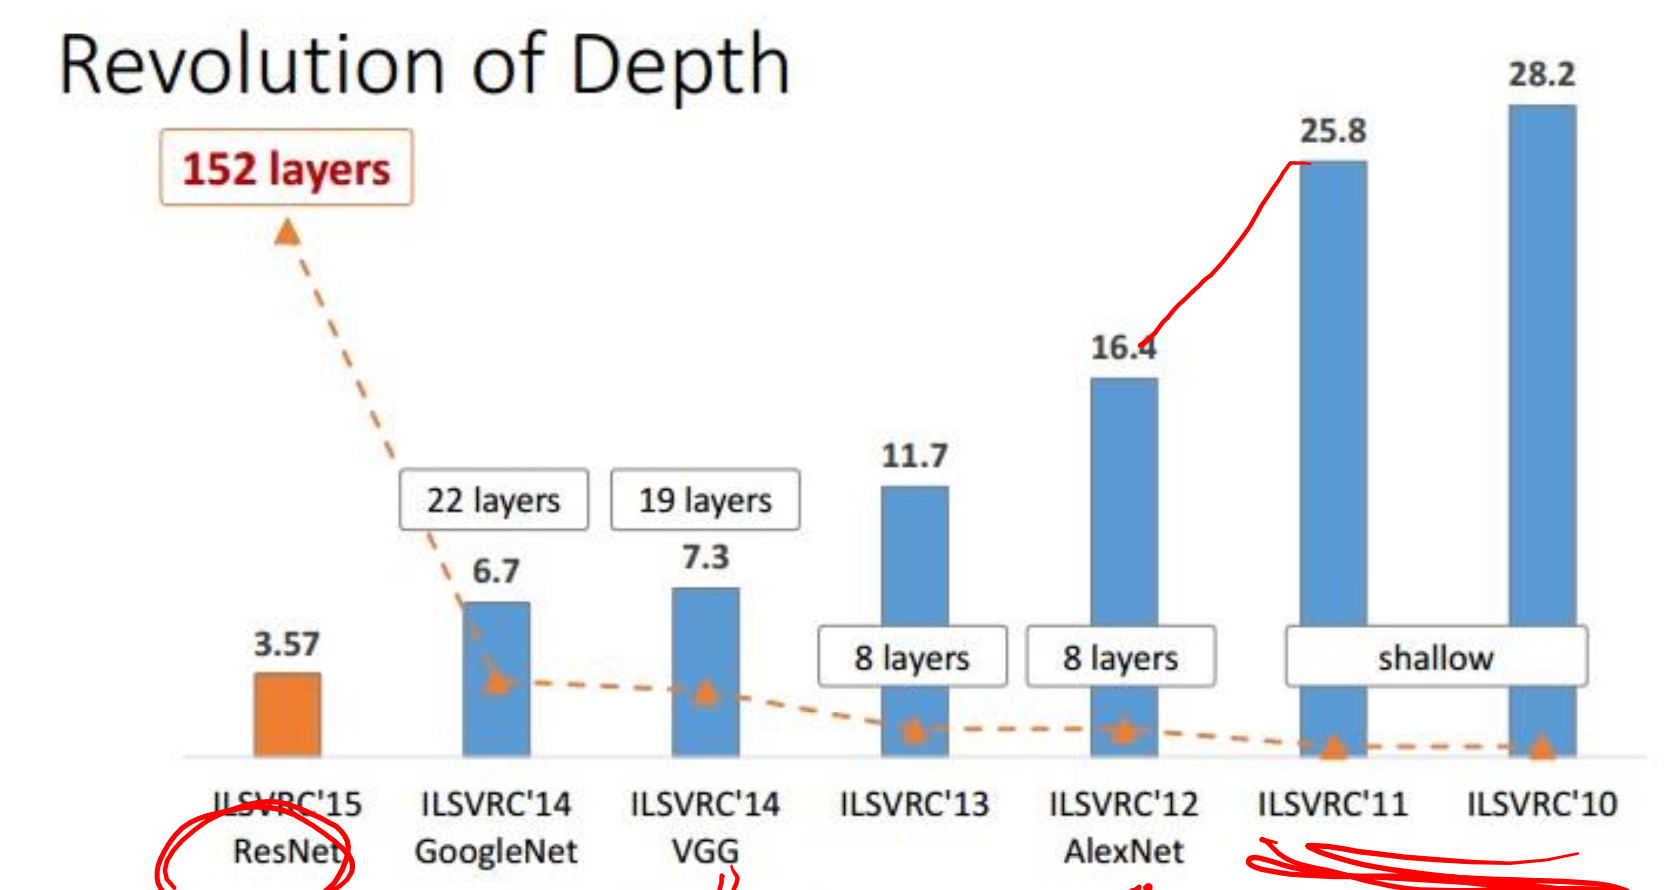
\includegraphics[width=\linewidth]{graphic/cnn-arch-evolution}
 		\captionof{figure}{Evolution of NN architecture}
	\end{Figure}
\end{comment}

\subsection{VGG vs. AlexNet}
less kernels/filters ($\downarrow$ params), more layers ($\uparrow$ perceptive field)\\
\begin{comment}
	Larger receptive field means that the net can respond to patterns that are larger spread apart.\\
	Each large filter, f.e. 11x11, can be represented using multiple 3x3 filters. The number of parameters for one 11x11 filter is 121, which is equal to using 5 3x3 filters with 45 parameters.\\
\end{comment}

\subsection{GoogleNet}
More layers, removed fully connected layer on the top.\\
\textbf{Inception:} use 1x1 conv. layers to reduce layer depth\\
\begin{comment}
	Because of small kernels and deep networks, the number of channels (depth) is going to be huge.
	Inception modules downsamples the activation maps, reducing the number of channels by convolution, and thus reducing the number of parameters.\\
	\Note{In addition, GoogLeNet uses auxiliary classification heads throughout the CNN, to make sure the gradients don't dry out.}\\
\end{comment}

\subsection{ResNet}
\textbf{Residual-Con:} Skips weight layers with residual connections.\\
\begin{comment}
	\Note{A deep network should at least perform as good as a shallow one (set all additional layers to identity).}\\
	This approach lead to the believe that failing to perform is an optimisation issue, not a design issue.\\
	ResNet one (drastic) downsampling and then residual layers.
	The "Ultra-deep" version is not used often, in general ResNet18 is used.\\
	
	\begin{Figure}
 		\centering
 		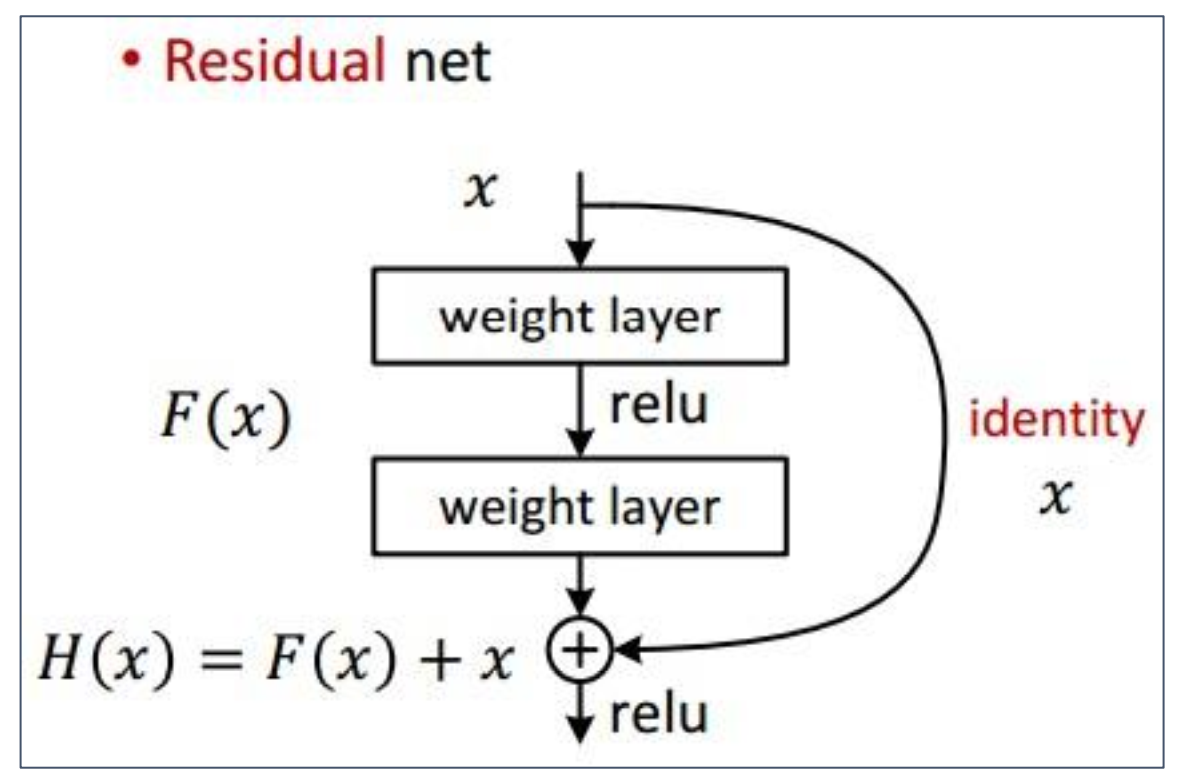
\includegraphics[width=\linewidth]{graphic/cnn-res-net}
 		\captionof{figure}{Evolution of NN architecture}
	\end{Figure}
\end{comment}












